\refstepcounter{section}
\section*{Lecture 27: Kadanoff's Block Spins}
\addcontentsline{toc}{section}{Lecture 27: Kadanoff's Block Spins}
In the previous lecture, we used an \textit{ad hoc} assumption of the thermodynamic quantitites being generalised homogenous functions. We now try to give a proper justification of why this turns out to be okay(ish)! For that, consider our favourite Ising model with $N$ spins, given by the corresponding Hamiltonian,
\begin{align*}
    \mathscr{H} = -J \sum\limits_{\avg{ij}} \sigma_i \sigma_j - h \sum\limits_{i}\sigma_i
\end{align*}
\begin{figure}[H]
    \centering
    

\tikzset{every picture/.style={line width=0.75pt}} %set default line width to 0.75pt        

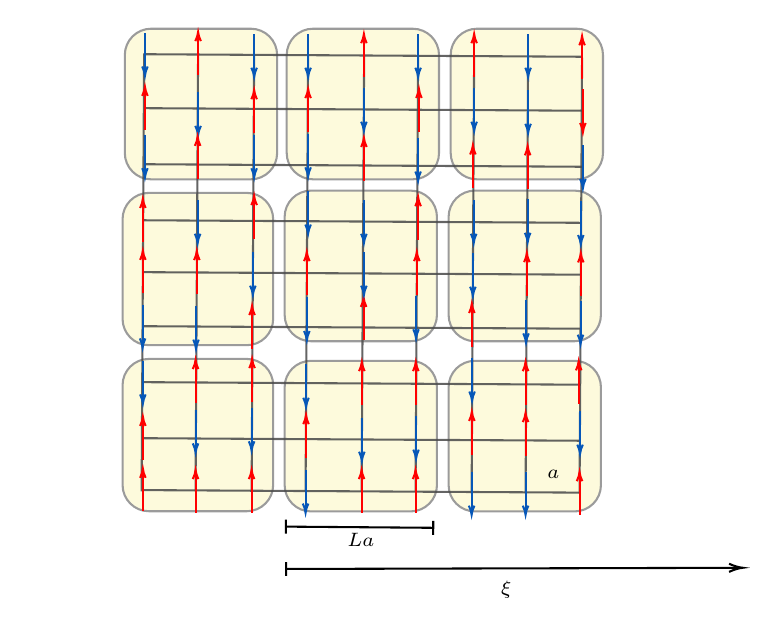
\begin{tikzpicture}[x=0.75pt,y=0.75pt,yscale=-1,xscale=1]
%uncomment if require: \path (0,395); %set diagram left start at 0, and has height of 395

%Flowchart: Alternative Process [id:dp539668995582457] 
\draw  [color={rgb, 255:red, 155; green, 155; blue, 155 }  ,draw opacity=1 ][fill={rgb, 255:red, 250; green, 243; blue, 176 }  ,fill opacity=0.44 ] (142.3,202.41) .. controls (142.3,195.39) and (147.99,189.71) .. (155,189.71) -- (202.99,189.71) .. controls (210.01,189.71) and (215.69,195.39) .. (215.69,202.41) -- (215.69,249.58) .. controls (215.69,256.59) and (210.01,262.28) .. (202.99,262.28) -- (155,262.28) .. controls (147.99,262.28) and (142.3,256.59) .. (142.3,249.58) -- cycle ;
%Flowchart: Alternative Process [id:dp2601694946136637] 
\draw  [color={rgb, 255:red, 155; green, 155; blue, 155 }  ,draw opacity=1 ][fill={rgb, 255:red, 250; green, 243; blue, 176 }  ,fill opacity=0.44 ] (142.3,120.41) .. controls (142.3,113.39) and (147.99,107.71) .. (155,107.71) -- (202.99,107.71) .. controls (210.01,107.71) and (215.69,113.39) .. (215.69,120.41) -- (215.69,167.58) .. controls (215.69,174.59) and (210.01,180.28) .. (202.99,180.28) -- (155,180.28) .. controls (147.99,180.28) and (142.3,174.59) .. (142.3,167.58) -- cycle ;
%Flowchart: Alternative Process [id:dp09620523975709283] 
\draw  [color={rgb, 255:red, 155; green, 155; blue, 155 }  ,draw opacity=1 ][fill={rgb, 255:red, 250; green, 243; blue, 176 }  ,fill opacity=0.44 ] (124.08,108.8) .. controls (131.09,108.8) and (136.78,114.48) .. (136.78,121.5) -- (136.78,169.49) .. controls (136.78,176.5) and (131.09,182.19) .. (124.08,182.19) -- (76.91,182.19) .. controls (69.9,182.19) and (64.21,176.5) .. (64.21,169.49) -- (64.21,121.5) .. controls (64.21,114.48) and (69.9,108.8) .. (76.91,108.8) -- cycle ;
%Flowchart: Alternative Process [id:dp2259248871998749] 
\draw  [color={rgb, 255:red, 155; green, 155; blue, 155 }  ,draw opacity=1 ][fill={rgb, 255:red, 250; green, 243; blue, 176 }  ,fill opacity=0.44 ] (124.08,188.8) .. controls (131.09,188.8) and (136.78,194.48) .. (136.78,201.5) -- (136.78,249.49) .. controls (136.78,256.5) and (131.09,262.19) .. (124.08,262.19) -- (76.91,262.19) .. controls (69.9,262.19) and (64.21,256.5) .. (64.21,249.49) -- (64.21,201.5) .. controls (64.21,194.48) and (69.9,188.8) .. (76.91,188.8) -- cycle ;
%Flowchart: Alternative Process [id:dp2360682514573128] 
\draw  [color={rgb, 255:red, 155; green, 155; blue, 155 }  ,draw opacity=1 ][fill={rgb, 255:red, 250; green, 243; blue, 176 }  ,fill opacity=0.44 ] (222.3,42.41) .. controls (222.3,35.39) and (227.99,29.71) .. (235,29.71) -- (282.99,29.71) .. controls (290.01,29.71) and (295.69,35.39) .. (295.69,42.41) -- (295.69,89.58) .. controls (295.69,96.59) and (290.01,102.28) .. (282.99,102.28) -- (235,102.28) .. controls (227.99,102.28) and (222.3,96.59) .. (222.3,89.58) -- cycle ;
%Flowchart: Alternative Process [id:dp3542787625094702] 
\draw  [color={rgb, 255:red, 155; green, 155; blue, 155 }  ,draw opacity=1 ][fill={rgb, 255:red, 250; green, 243; blue, 176 }  ,fill opacity=0.44 ] (221.3,120.41) .. controls (221.3,113.39) and (226.99,107.71) .. (234,107.71) -- (281.99,107.71) .. controls (289.01,107.71) and (294.69,113.39) .. (294.69,120.41) -- (294.69,167.58) .. controls (294.69,174.59) and (289.01,180.28) .. (281.99,180.28) -- (234,180.28) .. controls (226.99,180.28) and (221.3,174.59) .. (221.3,167.58) -- cycle ;
%Flowchart: Alternative Process [id:dp11107826982046776] 
\draw  [color={rgb, 255:red, 155; green, 155; blue, 155 }  ,draw opacity=1 ][fill={rgb, 255:red, 250; green, 243; blue, 176 }  ,fill opacity=0.44 ] (221.3,202.41) .. controls (221.3,195.39) and (226.99,189.71) .. (234,189.71) -- (281.99,189.71) .. controls (289.01,189.71) and (294.69,195.39) .. (294.69,202.41) -- (294.69,249.58) .. controls (294.69,256.59) and (289.01,262.28) .. (281.99,262.28) -- (234,262.28) .. controls (226.99,262.28) and (221.3,256.59) .. (221.3,249.58) -- cycle ;
%Flowchart: Alternative Process [id:dp47975033445161597] 
\draw  [color={rgb, 255:red, 155; green, 155; blue, 155 }  ,draw opacity=1 ][fill={rgb, 255:red, 250; green, 243; blue, 176 }  ,fill opacity=0.44 ] (143.3,42.41) .. controls (143.3,35.39) and (148.99,29.71) .. (156,29.71) -- (203.99,29.71) .. controls (211.01,29.71) and (216.69,35.39) .. (216.69,42.41) -- (216.69,89.58) .. controls (216.69,96.59) and (211.01,102.28) .. (203.99,102.28) -- (156,102.28) .. controls (148.99,102.28) and (143.3,96.59) .. (143.3,89.58) -- cycle ;
%Flowchart: Alternative Process [id:dp9006467305029361] 
\draw  [color={rgb, 255:red, 155; green, 155; blue, 155 }  ,draw opacity=1 ][fill={rgb, 255:red, 250; green, 243; blue, 176 }  ,fill opacity=0.44 ] (65.3,42.41) .. controls (65.3,35.39) and (70.99,29.71) .. (78,29.71) -- (125.99,29.71) .. controls (133.01,29.71) and (138.69,35.39) .. (138.69,42.41) -- (138.69,89.58) .. controls (138.69,96.59) and (133.01,102.28) .. (125.99,102.28) -- (78,102.28) .. controls (70.99,102.28) and (65.3,96.59) .. (65.3,89.58) -- cycle ;
%Straight Lines [id:da6085385907209341] 
\draw [color={rgb, 255:red, 74; green, 74; blue, 74 }  ,draw opacity=0.86 ]   (75,42) -- (286,43.22) ;
%Straight Lines [id:da6924449573297418] 
\draw [color={rgb, 255:red, 74; green, 74; blue, 74 }  ,draw opacity=0.86 ]   (75,68) -- (286,69.22) ;
%Straight Lines [id:da891977584262932] 
\draw [color={rgb, 255:red, 74; green, 74; blue, 74 }  ,draw opacity=0.86 ]   (285.61,43.61) -- (284.87,174.25) -- (284.39,253.61) ;
%Straight Lines [id:da20918906461082798] 
\draw [color={rgb, 255:red, 74; green, 74; blue, 74 }  ,draw opacity=0.86 ]   (100.61,41.61) -- (99.39,252.61) ;
%Straight Lines [id:da5801416510302981] 
\draw [color={rgb, 255:red, 74; green, 74; blue, 74 }  ,draw opacity=0.86 ]   (75,95) -- (286,96.22) ;
%Straight Lines [id:da12982854127633614] 
\draw [color={rgb, 255:red, 74; green, 74; blue, 74 }  ,draw opacity=0.86 ]   (74,122) -- (285,123.22) ;
%Straight Lines [id:da6502464141943719] 
\draw [color={rgb, 255:red, 74; green, 74; blue, 74 }  ,draw opacity=0.86 ]   (74,147) -- (285,148.22) ;
%Straight Lines [id:da2439670916493083] 
\draw [color={rgb, 255:red, 74; green, 74; blue, 74 }  ,draw opacity=0.86 ]   (73.87,173.04) -- (284.87,174.25) ;
%Straight Lines [id:da4279236592192597] 
\draw [color={rgb, 255:red, 74; green, 74; blue, 74 }  ,draw opacity=0.86 ]   (74,200) -- (285,201.22) ;
%Straight Lines [id:da3819887406014746] 
\draw [color={rgb, 255:red, 74; green, 74; blue, 74 }  ,draw opacity=0.86 ]   (74,227) -- (285,228.22) ;
%Straight Lines [id:da5239673463971988] 
\draw [color={rgb, 255:red, 74; green, 74; blue, 74 }  ,draw opacity=0.86 ]   (74,252) -- (285,253.22) ;
%Straight Lines [id:da47091028093753007] 
\draw [color={rgb, 255:red, 74; green, 74; blue, 74 }  ,draw opacity=0.86 ]   (74.61,41.61) -- (73.39,252.61) ;
%Straight Lines [id:da07343983668749199] 
\draw [color={rgb, 255:red, 74; green, 74; blue, 74 }  ,draw opacity=0.86 ]   (153.61,42.61) -- (152.39,252.61) ;
%Straight Lines [id:da6981339284016169] 
\draw [color={rgb, 255:red, 74; green, 74; blue, 74 }  ,draw opacity=0.86 ]   (127.61,42.61) -- (126.39,252.61) ;
%Straight Lines [id:da010793330718061322] 
\draw [color={rgb, 255:red, 74; green, 74; blue, 74 }  ,draw opacity=0.86 ]   (206.61,42.61) -- (205.39,252.61) ;
%Straight Lines [id:da08414306289963558] 
\draw [color={rgb, 255:red, 74; green, 74; blue, 74 }  ,draw opacity=0.86 ]   (180.61,42.61) -- (179.39,252.61) ;
%Straight Lines [id:da8675240410611694] 
\draw [color={rgb, 255:red, 74; green, 74; blue, 74 }  ,draw opacity=0.86 ]   (259.61,42.61) -- (258.39,253.61) ;
%Straight Lines [id:da10983364891380876] 
\draw [color={rgb, 255:red, 74; green, 74; blue, 74 }  ,draw opacity=0.86 ]   (233.61,42.61) -- (232.39,253.61) ;
%Straight Lines [id:da9363765597349243] 
\draw [color={rgb, 255:red, 255; green, 0; blue, 0 }  ,draw opacity=1 ]   (100.61,51.88) -- (100.61,33.33) ;
\draw [shift={(100.61,31.33)}, rotate = 90] [color={rgb, 255:red, 255; green, 0; blue, 0 }  ,draw opacity=1 ][line width=0.75]    (4.37,-1.32) .. controls (2.78,-0.56) and (1.32,-0.12) .. (0,0) .. controls (1.32,0.12) and (2.78,0.56) .. (4.37,1.32)   ;
%Straight Lines [id:da39368481093875096] 
\draw [color={rgb, 255:red, 255; green, 0; blue, 0 }  ,draw opacity=1 ]   (127.61,79.88) -- (127.61,61.33) ;
\draw [shift={(127.61,59.33)}, rotate = 90] [color={rgb, 255:red, 255; green, 0; blue, 0 }  ,draw opacity=1 ][line width=0.75]    (4.37,-1.32) .. controls (2.78,-0.56) and (1.32,-0.12) .. (0,0) .. controls (1.32,0.12) and (2.78,0.56) .. (4.37,1.32)   ;
%Straight Lines [id:da4664636997308226] 
\draw [color={rgb, 255:red, 255; green, 0; blue, 0 }  ,draw opacity=1 ]   (127.61,130.88) -- (127.61,112.33) ;
\draw [shift={(127.61,110.33)}, rotate = 90] [color={rgb, 255:red, 255; green, 0; blue, 0 }  ,draw opacity=1 ][line width=0.75]    (4.37,-1.32) .. controls (2.78,-0.56) and (1.32,-0.12) .. (0,0) .. controls (1.32,0.12) and (2.78,0.56) .. (4.37,1.32)   ;
%Straight Lines [id:da9232354030565457] 
\draw [color={rgb, 255:red, 255; green, 0; blue, 0 }  ,draw opacity=1 ]   (180.5,102.88) -- (180.5,84.33) ;
\draw [shift={(180.5,82.33)}, rotate = 90] [color={rgb, 255:red, 255; green, 0; blue, 0 }  ,draw opacity=1 ][line width=0.75]    (4.37,-1.32) .. controls (2.78,-0.56) and (1.32,-0.12) .. (0,0) .. controls (1.32,0.12) and (2.78,0.56) .. (4.37,1.32)   ;
%Straight Lines [id:da39095968430093075] 
\draw [color={rgb, 255:red, 255; green, 0; blue, 0 }  ,draw opacity=1 ]   (126.61,183.88) -- (126.61,165.33) ;
\draw [shift={(126.61,163.33)}, rotate = 90] [color={rgb, 255:red, 255; green, 0; blue, 0 }  ,draw opacity=1 ][line width=0.75]    (4.37,-1.32) .. controls (2.78,-0.56) and (1.32,-0.12) .. (0,0) .. controls (1.32,0.12) and (2.78,0.56) .. (4.37,1.32)   ;
%Straight Lines [id:da948590026689967] 
\draw [color={rgb, 255:red, 255; green, 0; blue, 0 }  ,draw opacity=1 ]   (179.5,210.88) -- (179.5,192.33) ;
\draw [shift={(179.5,190.33)}, rotate = 90] [color={rgb, 255:red, 255; green, 0; blue, 0 }  ,draw opacity=1 ][line width=0.75]    (4.37,-1.32) .. controls (2.78,-0.56) and (1.32,-0.12) .. (0,0) .. controls (1.32,0.12) and (2.78,0.56) .. (4.37,1.32)   ;
%Straight Lines [id:da8277836600347181] 
\draw [color={rgb, 255:red, 255; green, 0; blue, 0 }  ,draw opacity=1 ]   (232.5,182.88) -- (232.5,164.33) ;
\draw [shift={(232.5,162.33)}, rotate = 90] [color={rgb, 255:red, 255; green, 0; blue, 0 }  ,draw opacity=1 ][line width=0.75]    (4.37,-1.32) .. controls (2.78,-0.56) and (1.32,-0.12) .. (0,0) .. controls (1.32,0.12) and (2.78,0.56) .. (4.37,1.32)   ;
%Straight Lines [id:da28844065132295105] 
\draw [color={rgb, 255:red, 255; green, 0; blue, 0 }  ,draw opacity=1 ]   (284.39,263.88) -- (284.39,245.33) ;
\draw [shift={(284.39,243.33)}, rotate = 90] [color={rgb, 255:red, 255; green, 0; blue, 0 }  ,draw opacity=1 ][line width=0.75]    (4.37,-1.32) .. controls (2.78,-0.56) and (1.32,-0.12) .. (0,0) .. controls (1.32,0.12) and (2.78,0.56) .. (4.37,1.32)   ;
%Straight Lines [id:da11225313698749606] 
\draw [color={rgb, 255:red, 255; green, 0; blue, 0 }  ,draw opacity=1 ]   (74,157.28) -- (74,138.72) ;
\draw [shift={(74,136.72)}, rotate = 90] [color={rgb, 255:red, 255; green, 0; blue, 0 }  ,draw opacity=1 ][line width=0.75]    (4.37,-1.32) .. controls (2.78,-0.56) and (1.32,-0.12) .. (0,0) .. controls (1.32,0.12) and (2.78,0.56) .. (4.37,1.32)   ;
%Straight Lines [id:da31762019946690223] 
\draw [color={rgb, 255:red, 255; green, 0; blue, 0 }  ,draw opacity=1 ]   (259.39,106.88) -- (259.39,88.33) ;
\draw [shift={(259.39,86.33)}, rotate = 90] [color={rgb, 255:red, 255; green, 0; blue, 0 }  ,draw opacity=1 ][line width=0.75]    (4.37,-1.32) .. controls (2.78,-0.56) and (1.32,-0.12) .. (0,0) .. controls (1.32,0.12) and (2.78,0.56) .. (4.37,1.32)   ;
%Straight Lines [id:da3157253653989722] 
\draw [color={rgb, 255:red, 255; green, 0; blue, 0 }  ,draw opacity=1 ]   (74,262.28) -- (74,243.72) ;
\draw [shift={(74,241.72)}, rotate = 90] [color={rgb, 255:red, 255; green, 0; blue, 0 }  ,draw opacity=1 ][line width=0.75]    (4.37,-1.32) .. controls (2.78,-0.56) and (1.32,-0.12) .. (0,0) .. controls (1.32,0.12) and (2.78,0.56) .. (4.37,1.32)   ;
%Straight Lines [id:da16330853824616942] 
\draw [color={rgb, 255:red, 255; green, 0; blue, 0 }  ,draw opacity=1 ]   (153,157.88) -- (153,139.33) ;
\draw [shift={(153,137.33)}, rotate = 90] [color={rgb, 255:red, 255; green, 0; blue, 0 }  ,draw opacity=1 ][line width=0.75]    (4.37,-1.32) .. controls (2.78,-0.56) and (1.32,-0.12) .. (0,0) .. controls (1.32,0.12) and (2.78,0.56) .. (4.37,1.32)   ;
%Straight Lines [id:da2083314881984173] 
\draw [color={rgb, 255:red, 255; green, 0; blue, 0 }  ,draw opacity=1 ]   (126.39,262.88) -- (126.39,244.33) ;
\draw [shift={(126.39,242.33)}, rotate = 90] [color={rgb, 255:red, 255; green, 0; blue, 0 }  ,draw opacity=1 ][line width=0.75]    (4.37,-1.32) .. controls (2.78,-0.56) and (1.32,-0.12) .. (0,0) .. controls (1.32,0.12) and (2.78,0.56) .. (4.37,1.32)   ;
%Straight Lines [id:da5279467991318754] 
\draw [color={rgb, 255:red, 255; green, 0; blue, 0 }  ,draw opacity=1 ]   (99.39,209.88) -- (99.39,191.33) ;
\draw [shift={(99.39,189.33)}, rotate = 90] [color={rgb, 255:red, 255; green, 0; blue, 0 }  ,draw opacity=1 ][line width=0.75]    (4.37,-1.32) .. controls (2.78,-0.56) and (1.32,-0.12) .. (0,0) .. controls (1.32,0.12) and (2.78,0.56) .. (4.37,1.32)   ;
%Straight Lines [id:da6688297815131616] 
\draw [color={rgb, 255:red, 255; green, 0; blue, 0 }  ,draw opacity=1 ]   (180.5,52.88) -- (180.5,34.33) ;
\draw [shift={(180.5,32.33)}, rotate = 90] [color={rgb, 255:red, 255; green, 0; blue, 0 }  ,draw opacity=1 ][line width=0.75]    (4.37,-1.32) .. controls (2.78,-0.56) and (1.32,-0.12) .. (0,0) .. controls (1.32,0.12) and (2.78,0.56) .. (4.37,1.32)   ;
%Straight Lines [id:da7541872396131746] 
\draw [color={rgb, 255:red, 255; green, 0; blue, 0 }  ,draw opacity=1 ]   (206,157.88) -- (206,139.33) ;
\draw [shift={(206,137.33)}, rotate = 90] [color={rgb, 255:red, 255; green, 0; blue, 0 }  ,draw opacity=1 ][line width=0.75]    (4.37,-1.32) .. controls (2.78,-0.56) and (1.32,-0.12) .. (0,0) .. controls (1.32,0.12) and (2.78,0.56) .. (4.37,1.32)   ;
%Straight Lines [id:da23221817830699298] 
\draw [color={rgb, 255:red, 255; green, 0; blue, 0 }  ,draw opacity=1 ]   (75,78.28) -- (75,59.72) ;
\draw [shift={(75,57.72)}, rotate = 90] [color={rgb, 255:red, 255; green, 0; blue, 0 }  ,draw opacity=1 ][line width=0.75]    (4.37,-1.32) .. controls (2.78,-0.56) and (1.32,-0.12) .. (0,0) .. controls (1.32,0.12) and (2.78,0.56) .. (4.37,1.32)   ;
%Straight Lines [id:da6331376023437454] 
\draw [color={rgb, 255:red, 255; green, 0; blue, 0 }  ,draw opacity=1 ]   (205.39,262.88) -- (205.39,244.33) ;
\draw [shift={(205.39,242.33)}, rotate = 90] [color={rgb, 255:red, 255; green, 0; blue, 0 }  ,draw opacity=1 ][line width=0.75]    (4.37,-1.32) .. controls (2.78,-0.56) and (1.32,-0.12) .. (0,0) .. controls (1.32,0.12) and (2.78,0.56) .. (4.37,1.32)   ;
%Straight Lines [id:da9362887410756234] 
\draw [color={rgb, 255:red, 255; green, 0; blue, 0 }  ,draw opacity=1 ]   (258.39,210.88) -- (258.39,192.33) ;
\draw [shift={(258.39,190.33)}, rotate = 90] [color={rgb, 255:red, 255; green, 0; blue, 0 }  ,draw opacity=1 ][line width=0.75]    (4.37,-1.32) .. controls (2.78,-0.56) and (1.32,-0.12) .. (0,0) .. controls (1.32,0.12) and (2.78,0.56) .. (4.37,1.32)   ;
%Straight Lines [id:da2435747911504541] 
\draw [color={rgb, 255:red, 255; green, 0; blue, 0 }  ,draw opacity=1 ]   (285.61,53.88) -- (285.61,35.33) ;
\draw [shift={(285.61,33.33)}, rotate = 90] [color={rgb, 255:red, 255; green, 0; blue, 0 }  ,draw opacity=1 ][line width=0.75]    (4.37,-1.32) .. controls (2.78,-0.56) and (1.32,-0.12) .. (0,0) .. controls (1.32,0.12) and (2.78,0.56) .. (4.37,1.32)   ;
%Straight Lines [id:da8305111780112114] 
\draw [color={rgb, 255:red, 6; green, 87; blue, 184 }  ,draw opacity=1 ][fill={rgb, 255:red, 11; green, 89; blue, 173 }  ,fill opacity=1 ]   (206.61,32.33) -- (206.61,50.88) ;
\draw [shift={(206.61,52.88)}, rotate = 270] [color={rgb, 255:red, 6; green, 87; blue, 184 }  ,draw opacity=1 ][line width=0.75]    (4.37,-1.32) .. controls (2.78,-0.56) and (1.32,-0.12) .. (0,0) .. controls (1.32,0.12) and (2.78,0.56) .. (4.37,1.32)   ;
%Straight Lines [id:da07276828198409291] 
\draw [color={rgb, 255:red, 6; green, 87; blue, 184 }  ,draw opacity=1 ][fill={rgb, 255:red, 11; green, 89; blue, 173 }  ,fill opacity=1 ]   (153.61,80.33) -- (153.61,98.88) ;
\draw [shift={(153.61,100.88)}, rotate = 270] [color={rgb, 255:red, 6; green, 87; blue, 184 }  ,draw opacity=1 ][line width=0.75]    (4.37,-1.32) .. controls (2.78,-0.56) and (1.32,-0.12) .. (0,0) .. controls (1.32,0.12) and (2.78,0.56) .. (4.37,1.32)   ;
%Straight Lines [id:da32562585007828904] 
\draw [color={rgb, 255:red, 6; green, 87; blue, 184 }  ,draw opacity=1 ][fill={rgb, 255:red, 11; green, 89; blue, 173 }  ,fill opacity=1 ]   (100.61,60.33) -- (100.61,78.88) ;
\draw [shift={(100.61,80.88)}, rotate = 270] [color={rgb, 255:red, 6; green, 87; blue, 184 }  ,draw opacity=1 ][line width=0.75]    (4.37,-1.32) .. controls (2.78,-0.56) and (1.32,-0.12) .. (0,0) .. controls (1.32,0.12) and (2.78,0.56) .. (4.37,1.32)   ;
%Straight Lines [id:da4926525224998506] 
\draw [color={rgb, 255:red, 6; green, 87; blue, 184 }  ,draw opacity=1 ][fill={rgb, 255:red, 11; green, 89; blue, 173 }  ,fill opacity=1 ]   (259.61,32.33) -- (259.61,50.88) ;
\draw [shift={(259.61,52.88)}, rotate = 270] [color={rgb, 255:red, 6; green, 87; blue, 184 }  ,draw opacity=1 ][line width=0.75]    (4.37,-1.32) .. controls (2.78,-0.56) and (1.32,-0.12) .. (0,0) .. controls (1.32,0.12) and (2.78,0.56) .. (4.37,1.32)   ;
%Straight Lines [id:da11800360428868928] 
\draw [color={rgb, 255:red, 6; green, 87; blue, 184 }  ,draw opacity=1 ][fill={rgb, 255:red, 11; green, 89; blue, 173 }  ,fill opacity=1 ]   (180.5,112.33) -- (180.5,130.88) ;
\draw [shift={(180.5,132.88)}, rotate = 270] [color={rgb, 255:red, 6; green, 87; blue, 184 }  ,draw opacity=1 ][line width=0.75]    (4.37,-1.32) .. controls (2.78,-0.56) and (1.32,-0.12) .. (0,0) .. controls (1.32,0.12) and (2.78,0.56) .. (4.37,1.32)   ;
%Straight Lines [id:da9214179605726955] 
\draw [color={rgb, 255:red, 6; green, 87; blue, 184 }  ,draw opacity=1 ][fill={rgb, 255:red, 11; green, 89; blue, 173 }  ,fill opacity=1 ]   (153.61,107.88) -- (153.61,126.43) ;
\draw [shift={(153.61,128.43)}, rotate = 270] [color={rgb, 255:red, 6; green, 87; blue, 184 }  ,draw opacity=1 ][line width=0.75]    (4.37,-1.32) .. controls (2.78,-0.56) and (1.32,-0.12) .. (0,0) .. controls (1.32,0.12) and (2.78,0.56) .. (4.37,1.32)   ;
%Straight Lines [id:da6063137798520921] 
\draw [color={rgb, 255:red, 6; green, 87; blue, 184 }  ,draw opacity=1 ][fill={rgb, 255:red, 11; green, 89; blue, 173 }  ,fill opacity=1 ]   (285,112.94) -- (285,131.49) ;
\draw [shift={(285,133.49)}, rotate = 270] [color={rgb, 255:red, 6; green, 87; blue, 184 }  ,draw opacity=1 ][line width=0.75]    (4.37,-1.32) .. controls (2.78,-0.56) and (1.32,-0.12) .. (0,0) .. controls (1.32,0.12) and (2.78,0.56) .. (4.37,1.32)   ;
%Straight Lines [id:da8160422083498822] 
\draw [color={rgb, 255:red, 6; green, 87; blue, 184 }  ,draw opacity=1 ][fill={rgb, 255:red, 11; green, 89; blue, 173 }  ,fill opacity=1 ]   (286,85.94) -- (286,104.49) ;
\draw [shift={(286,106.49)}, rotate = 270] [color={rgb, 255:red, 6; green, 87; blue, 184 }  ,draw opacity=1 ][line width=0.75]    (4.37,-1.32) .. controls (2.78,-0.56) and (1.32,-0.12) .. (0,0) .. controls (1.32,0.12) and (2.78,0.56) .. (4.37,1.32)   ;
%Straight Lines [id:da9788208025632859] 
\draw [color={rgb, 255:red, 6; green, 87; blue, 184 }  ,draw opacity=1 ][fill={rgb, 255:red, 11; green, 89; blue, 173 }  ,fill opacity=1 ]   (205.61,158.33) -- (205.61,176.88) ;
\draw [shift={(205.61,178.88)}, rotate = 270] [color={rgb, 255:red, 6; green, 87; blue, 184 }  ,draw opacity=1 ][line width=0.75]    (4.37,-1.32) .. controls (2.78,-0.56) and (1.32,-0.12) .. (0,0) .. controls (1.32,0.12) and (2.78,0.56) .. (4.37,1.32)   ;
%Straight Lines [id:da58910835993692] 
\draw [color={rgb, 255:red, 6; green, 87; blue, 184 }  ,draw opacity=1 ][fill={rgb, 255:red, 11; green, 89; blue, 173 }  ,fill opacity=1 ]   (152.61,191.33) -- (152.61,209.88) ;
\draw [shift={(152.61,211.88)}, rotate = 270] [color={rgb, 255:red, 6; green, 87; blue, 184 }  ,draw opacity=1 ][line width=0.75]    (4.37,-1.32) .. controls (2.78,-0.56) and (1.32,-0.12) .. (0,0) .. controls (1.32,0.12) and (2.78,0.56) .. (4.37,1.32)   ;
%Straight Lines [id:da48330849628712236] 
\draw [color={rgb, 255:red, 6; green, 87; blue, 184 }  ,draw opacity=1 ][fill={rgb, 255:red, 11; green, 89; blue, 173 }  ,fill opacity=1 ]   (153,159.16) -- (153,177.71) ;
\draw [shift={(153,179.71)}, rotate = 270] [color={rgb, 255:red, 6; green, 87; blue, 184 }  ,draw opacity=1 ][line width=0.75]    (4.37,-1.32) .. controls (2.78,-0.56) and (1.32,-0.12) .. (0,0) .. controls (1.32,0.12) and (2.78,0.56) .. (4.37,1.32)   ;
%Straight Lines [id:da739054033844131] 
\draw [color={rgb, 255:red, 6; green, 87; blue, 184 }  ,draw opacity=1 ][fill={rgb, 255:red, 11; green, 89; blue, 173 }  ,fill opacity=1 ]   (232.39,243.33) -- (232.39,261.88) ;
\draw [shift={(232.39,263.88)}, rotate = 270] [color={rgb, 255:red, 6; green, 87; blue, 184 }  ,draw opacity=1 ][line width=0.75]    (4.37,-1.32) .. controls (2.78,-0.56) and (1.32,-0.12) .. (0,0) .. controls (1.32,0.12) and (2.78,0.56) .. (4.37,1.32)   ;
%Straight Lines [id:da6656636313735281] 
\draw [color={rgb, 255:red, 6; green, 87; blue, 184 }  ,draw opacity=1 ][fill={rgb, 255:red, 11; green, 89; blue, 173 }  ,fill opacity=1 ]   (258.39,243.33) -- (258.39,261.88) ;
\draw [shift={(258.39,263.88)}, rotate = 270] [color={rgb, 255:red, 6; green, 87; blue, 184 }  ,draw opacity=1 ][line width=0.75]    (4.37,-1.32) .. controls (2.78,-0.56) and (1.32,-0.12) .. (0,0) .. controls (1.32,0.12) and (2.78,0.56) .. (4.37,1.32)   ;
%Straight Lines [id:da7290596971505342] 
\draw [color={rgb, 255:red, 6; green, 87; blue, 184 }  ,draw opacity=1 ][fill={rgb, 255:red, 11; green, 89; blue, 173 }  ,fill opacity=1 ]   (152.39,242.33) -- (152.39,260.88) ;
\draw [shift={(152.39,262.88)}, rotate = 270] [color={rgb, 255:red, 6; green, 87; blue, 184 }  ,draw opacity=1 ][line width=0.75]    (4.37,-1.32) .. controls (2.78,-0.56) and (1.32,-0.12) .. (0,0) .. controls (1.32,0.12) and (2.78,0.56) .. (4.37,1.32)   ;
%Straight Lines [id:da44385852568448714] 
\draw [color={rgb, 255:red, 6; green, 87; blue, 184 }  ,draw opacity=1 ][fill={rgb, 255:red, 11; green, 89; blue, 173 }  ,fill opacity=1 ]   (99.39,213.33) -- (99.39,231.88) ;
\draw [shift={(99.39,233.88)}, rotate = 270] [color={rgb, 255:red, 6; green, 87; blue, 184 }  ,draw opacity=1 ][line width=0.75]    (4.37,-1.32) .. controls (2.78,-0.56) and (1.32,-0.12) .. (0,0) .. controls (1.32,0.12) and (2.78,0.56) .. (4.37,1.32)   ;
%Straight Lines [id:da965028171623036] 
\draw [color={rgb, 255:red, 6; green, 87; blue, 184 }  ,draw opacity=1 ][fill={rgb, 255:red, 11; green, 89; blue, 173 }  ,fill opacity=1 ]   (127.61,32.33) -- (127.61,50.88) ;
\draw [shift={(127.61,52.88)}, rotate = 270] [color={rgb, 255:red, 6; green, 87; blue, 184 }  ,draw opacity=1 ][line width=0.75]    (4.37,-1.32) .. controls (2.78,-0.56) and (1.32,-0.12) .. (0,0) .. controls (1.32,0.12) and (2.78,0.56) .. (4.37,1.32)   ;
%Straight Lines [id:da8352102628632495] 
\draw [color={rgb, 255:red, 6; green, 87; blue, 184 }  ,draw opacity=1 ][fill={rgb, 255:red, 11; green, 89; blue, 173 }  ,fill opacity=1 ]   (153.61,32.33) -- (153.61,50.88) ;
\draw [shift={(153.61,52.88)}, rotate = 270] [color={rgb, 255:red, 6; green, 87; blue, 184 }  ,draw opacity=1 ][line width=0.75]    (4.37,-1.32) .. controls (2.78,-0.56) and (1.32,-0.12) .. (0,0) .. controls (1.32,0.12) and (2.78,0.56) .. (4.37,1.32)   ;
%Straight Lines [id:da8510524314410525] 
\draw [color={rgb, 255:red, 6; green, 87; blue, 184 }  ,draw opacity=1 ][fill={rgb, 255:red, 11; green, 89; blue, 173 }  ,fill opacity=1 ]   (100.39,112.33) -- (100.39,130.88) ;
\draw [shift={(100.39,132.88)}, rotate = 270] [color={rgb, 255:red, 6; green, 87; blue, 184 }  ,draw opacity=1 ][line width=0.75]    (4.37,-1.32) .. controls (2.78,-0.56) and (1.32,-0.12) .. (0,0) .. controls (1.32,0.12) and (2.78,0.56) .. (4.37,1.32)   ;
%Straight Lines [id:da7505915064171886] 
\draw [color={rgb, 255:red, 6; green, 87; blue, 184 }  ,draw opacity=1 ][fill={rgb, 255:red, 11; green, 89; blue, 173 }  ,fill opacity=1 ]   (73.87,162.76) -- (73.87,181.31) ;
\draw [shift={(73.87,183.31)}, rotate = 270] [color={rgb, 255:red, 6; green, 87; blue, 184 }  ,draw opacity=1 ][line width=0.75]    (4.37,-1.32) .. controls (2.78,-0.56) and (1.32,-0.12) .. (0,0) .. controls (1.32,0.12) and (2.78,0.56) .. (4.37,1.32)   ;
%Straight Lines [id:da32614887876645504] 
\draw [color={rgb, 255:red, 6; green, 87; blue, 184 }  ,draw opacity=1 ][fill={rgb, 255:red, 11; green, 89; blue, 173 }  ,fill opacity=1 ]   (74,189.72) -- (74,208.28) ;
\draw [shift={(74,210.28)}, rotate = 270] [color={rgb, 255:red, 6; green, 87; blue, 184 }  ,draw opacity=1 ][line width=0.75]    (4.37,-1.32) .. controls (2.78,-0.56) and (1.32,-0.12) .. (0,0) .. controls (1.32,0.12) and (2.78,0.56) .. (4.37,1.32)   ;
%Straight Lines [id:da21688651488691713] 
\draw [color={rgb, 255:red, 6; green, 87; blue, 184 }  ,draw opacity=1 ][fill={rgb, 255:red, 11; green, 89; blue, 173 }  ,fill opacity=1 ]   (233.39,112.33) -- (233.39,130.88) ;
\draw [shift={(233.39,132.88)}, rotate = 270] [color={rgb, 255:red, 6; green, 87; blue, 184 }  ,draw opacity=1 ][line width=0.75]    (4.37,-1.32) .. controls (2.78,-0.56) and (1.32,-0.12) .. (0,0) .. controls (1.32,0.12) and (2.78,0.56) .. (4.37,1.32)   ;
%Straight Lines [id:da3426262249981471] 
\draw [color={rgb, 255:red, 6; green, 87; blue, 184 }  ,draw opacity=1 ][fill={rgb, 255:red, 11; green, 89; blue, 173 }  ,fill opacity=1 ]   (284.63,213.93) -- (284.63,232.48) ;
\draw [shift={(284.63,234.48)}, rotate = 270] [color={rgb, 255:red, 6; green, 87; blue, 184 }  ,draw opacity=1 ][line width=0.75]    (4.37,-1.32) .. controls (2.78,-0.56) and (1.32,-0.12) .. (0,0) .. controls (1.32,0.12) and (2.78,0.56) .. (4.37,1.32)   ;
%Straight Lines [id:da5023648938482219] 
\draw [color={rgb, 255:red, 6; green, 87; blue, 184 }  ,draw opacity=1 ][fill={rgb, 255:red, 11; green, 89; blue, 173 }  ,fill opacity=1 ]   (126.39,212.33) -- (126.39,230.88) ;
\draw [shift={(126.39,232.88)}, rotate = 270] [color={rgb, 255:red, 6; green, 87; blue, 184 }  ,draw opacity=1 ][line width=0.75]    (4.37,-1.32) .. controls (2.78,-0.56) and (1.32,-0.12) .. (0,0) .. controls (1.32,0.12) and (2.78,0.56) .. (4.37,1.32)   ;
%Straight Lines [id:da6222930208105527] 
\draw [color={rgb, 255:red, 6; green, 87; blue, 184 }  ,draw opacity=1 ][fill={rgb, 255:red, 11; green, 89; blue, 173 }  ,fill opacity=1 ]   (75,31.72) -- (75,50.28) ;
\draw [shift={(75,52.28)}, rotate = 270] [color={rgb, 255:red, 6; green, 87; blue, 184 }  ,draw opacity=1 ][line width=0.75]    (4.37,-1.32) .. controls (2.78,-0.56) and (1.32,-0.12) .. (0,0) .. controls (1.32,0.12) and (2.78,0.56) .. (4.37,1.32)   ;
%Straight Lines [id:da5943472704807374] 
\draw [color={rgb, 255:red, 255; green, 0; blue, 0 }  ,draw opacity=1 ]   (233.61,34.33) -- (233.61,52.88) ;
\draw [shift={(233.61,32.33)}, rotate = 90] [color={rgb, 255:red, 255; green, 0; blue, 0 }  ,draw opacity=1 ][line width=0.75]    (4.37,-1.32) .. controls (2.78,-0.56) and (1.32,-0.12) .. (0,0) .. controls (1.32,0.12) and (2.78,0.56) .. (4.37,1.32)   ;
%Straight Lines [id:da8039813665703605] 
\draw [color={rgb, 255:red, 255; green, 0; blue, 0 }  ,draw opacity=1 ]   (286,58.94) -- (286,77.49) ;
\draw [shift={(286,79.49)}, rotate = 270] [color={rgb, 255:red, 255; green, 0; blue, 0 }  ,draw opacity=1 ][line width=0.75]    (4.37,-1.32) .. controls (2.78,-0.56) and (1.32,-0.12) .. (0,0) .. controls (1.32,0.12) and (2.78,0.56) .. (4.37,1.32)   ;
%Straight Lines [id:da8149403927499458] 
\draw [color={rgb, 255:red, 255; green, 0; blue, 0 }  ,draw opacity=1 ]   (284,191.94) -- (284,210.49) ;
\draw [shift={(284,189.94)}, rotate = 90] [color={rgb, 255:red, 255; green, 0; blue, 0 }  ,draw opacity=1 ][line width=0.75]    (4.37,-1.32) .. controls (2.78,-0.56) and (1.32,-0.12) .. (0,0) .. controls (1.32,0.12) and (2.78,0.56) .. (4.37,1.32)   ;
%Straight Lines [id:da4658559692834111] 
\draw [color={rgb, 255:red, 255; green, 0; blue, 0 }  ,draw opacity=1 ]   (285,139.94) -- (285,158.49) ;
\draw [shift={(285,137.94)}, rotate = 90] [color={rgb, 255:red, 255; green, 0; blue, 0 }  ,draw opacity=1 ][line width=0.75]    (4.37,-1.32) .. controls (2.78,-0.56) and (1.32,-0.12) .. (0,0) .. controls (1.32,0.12) and (2.78,0.56) .. (4.37,1.32)   ;
%Straight Lines [id:da42982397759857716] 
\draw [color={rgb, 255:red, 255; green, 0; blue, 0 }  ,draw opacity=1 ]   (259,139.83) -- (259,158.38) ;
\draw [shift={(259,137.83)}, rotate = 90] [color={rgb, 255:red, 255; green, 0; blue, 0 }  ,draw opacity=1 ][line width=0.75]    (4.37,-1.32) .. controls (2.78,-0.56) and (1.32,-0.12) .. (0,0) .. controls (1.32,0.12) and (2.78,0.56) .. (4.37,1.32)   ;
%Straight Lines [id:da37434994392813614] 
\draw [color={rgb, 255:red, 255; green, 0; blue, 0 }  ,draw opacity=1 ]   (100,138.83) -- (100,157.38) ;
\draw [shift={(100,136.83)}, rotate = 90] [color={rgb, 255:red, 255; green, 0; blue, 0 }  ,draw opacity=1 ][line width=0.75]    (4.37,-1.32) .. controls (2.78,-0.56) and (1.32,-0.12) .. (0,0) .. controls (1.32,0.12) and (2.78,0.56) .. (4.37,1.32)   ;
%Straight Lines [id:da10999561167037797] 
\draw [color={rgb, 255:red, 255; green, 0; blue, 0 }  ,draw opacity=1 ]   (179.39,244.33) -- (179.39,262.88) ;
\draw [shift={(179.39,242.33)}, rotate = 90] [color={rgb, 255:red, 255; green, 0; blue, 0 }  ,draw opacity=1 ][line width=0.75]    (4.37,-1.32) .. controls (2.78,-0.56) and (1.32,-0.12) .. (0,0) .. controls (1.32,0.12) and (2.78,0.56) .. (4.37,1.32)   ;
%Straight Lines [id:da5588137387847913] 
\draw [color={rgb, 255:red, 255; green, 0; blue, 0 }  ,draw opacity=1 ]   (233,87.94) -- (233,106.49) ;
\draw [shift={(233,85.94)}, rotate = 90] [color={rgb, 255:red, 255; green, 0; blue, 0 }  ,draw opacity=1 ][line width=0.75]    (4.37,-1.32) .. controls (2.78,-0.56) and (1.32,-0.12) .. (0,0) .. controls (1.32,0.12) and (2.78,0.56) .. (4.37,1.32)   ;
%Straight Lines [id:da8547749109733949] 
\draw [color={rgb, 255:red, 6; green, 87; blue, 184 }  ,draw opacity=1 ][fill={rgb, 255:red, 11; green, 89; blue, 173 }  ,fill opacity=1 ]   (233.61,58.33) -- (233.61,76.88) ;
\draw [shift={(233.61,78.88)}, rotate = 270] [color={rgb, 255:red, 6; green, 87; blue, 184 }  ,draw opacity=1 ][line width=0.75]    (4.37,-1.32) .. controls (2.78,-0.56) and (1.32,-0.12) .. (0,0) .. controls (1.32,0.12) and (2.78,0.56) .. (4.37,1.32)   ;
%Straight Lines [id:da9601769330850084] 
\draw [color={rgb, 255:red, 6; green, 87; blue, 184 }  ,draw opacity=1 ][fill={rgb, 255:red, 11; green, 89; blue, 173 }  ,fill opacity=1 ]   (259.61,59.33) -- (259.61,77.88) ;
\draw [shift={(259.61,79.88)}, rotate = 270] [color={rgb, 255:red, 6; green, 87; blue, 184 }  ,draw opacity=1 ][line width=0.75]    (4.37,-1.32) .. controls (2.78,-0.56) and (1.32,-0.12) .. (0,0) .. controls (1.32,0.12) and (2.78,0.56) .. (4.37,1.32)   ;
%Straight Lines [id:da2577309820808784] 
\draw [color={rgb, 255:red, 6; green, 87; blue, 184 }  ,draw opacity=1 ][fill={rgb, 255:red, 11; green, 89; blue, 173 }  ,fill opacity=1 ]   (75,80.72) -- (75,99.28) ;
\draw [shift={(75,101.28)}, rotate = 270] [color={rgb, 255:red, 6; green, 87; blue, 184 }  ,draw opacity=1 ][line width=0.75]    (4.37,-1.32) .. controls (2.78,-0.56) and (1.32,-0.12) .. (0,0) .. controls (1.32,0.12) and (2.78,0.56) .. (4.37,1.32)   ;
%Straight Lines [id:da8867498811795536] 
\draw [color={rgb, 255:red, 6; green, 87; blue, 184 }  ,draw opacity=1 ][fill={rgb, 255:red, 11; green, 89; blue, 173 }  ,fill opacity=1 ]   (127,137.33) -- (127,155.88) ;
\draw [shift={(127,157.88)}, rotate = 270] [color={rgb, 255:red, 6; green, 87; blue, 184 }  ,draw opacity=1 ][line width=0.75]    (4.37,-1.32) .. controls (2.78,-0.56) and (1.32,-0.12) .. (0,0) .. controls (1.32,0.12) and (2.78,0.56) .. (4.37,1.32)   ;
%Straight Lines [id:da37725244806903124] 
\draw [color={rgb, 255:red, 6; green, 87; blue, 184 }  ,draw opacity=1 ][fill={rgb, 255:red, 11; green, 89; blue, 173 }  ,fill opacity=1 ]   (99.61,163.33) -- (99.61,181.88) ;
\draw [shift={(99.61,183.88)}, rotate = 270] [color={rgb, 255:red, 6; green, 87; blue, 184 }  ,draw opacity=1 ][line width=0.75]    (4.37,-1.32) .. controls (2.78,-0.56) and (1.32,-0.12) .. (0,0) .. controls (1.32,0.12) and (2.78,0.56) .. (4.37,1.32)   ;
%Straight Lines [id:da8540953928494429] 
\draw [color={rgb, 255:red, 255; green, 0; blue, 0 }  ,draw opacity=1 ]   (205.5,210.88) -- (205.5,192.33) ;
\draw [shift={(205.5,190.33)}, rotate = 90] [color={rgb, 255:red, 255; green, 0; blue, 0 }  ,draw opacity=1 ][line width=0.75]    (4.37,-1.32) .. controls (2.78,-0.56) and (1.32,-0.12) .. (0,0) .. controls (1.32,0.12) and (2.78,0.56) .. (4.37,1.32)   ;
%Straight Lines [id:da537197002126827] 
\draw [color={rgb, 255:red, 255; green, 0; blue, 0 }  ,draw opacity=1 ]   (100.39,102.33) -- (100.39,83.78) ;
\draw [shift={(100.39,81.78)}, rotate = 90] [color={rgb, 255:red, 255; green, 0; blue, 0 }  ,draw opacity=1 ][line width=0.75]    (4.37,-1.32) .. controls (2.78,-0.56) and (1.32,-0.12) .. (0,0) .. controls (1.32,0.12) and (2.78,0.56) .. (4.37,1.32)   ;
%Straight Lines [id:da290101568592946] 
\draw [color={rgb, 255:red, 255; green, 0; blue, 0 }  ,draw opacity=1 ]   (126.61,209.43) -- (126.61,190.88) ;
\draw [shift={(126.61,188.88)}, rotate = 90] [color={rgb, 255:red, 255; green, 0; blue, 0 }  ,draw opacity=1 ][line width=0.75]    (4.37,-1.32) .. controls (2.78,-0.56) and (1.32,-0.12) .. (0,0) .. controls (1.32,0.12) and (2.78,0.56) .. (4.37,1.32)   ;
%Straight Lines [id:da29647749474326324] 
\draw [color={rgb, 255:red, 255; green, 0; blue, 0 }  ,draw opacity=1 ]   (232.5,234.88) -- (232.5,216.33) ;
\draw [shift={(232.5,214.33)}, rotate = 90] [color={rgb, 255:red, 255; green, 0; blue, 0 }  ,draw opacity=1 ][line width=0.75]    (4.37,-1.32) .. controls (2.78,-0.56) and (1.32,-0.12) .. (0,0) .. controls (1.32,0.12) and (2.78,0.56) .. (4.37,1.32)   ;
%Straight Lines [id:da3052060846761173] 
\draw [color={rgb, 255:red, 255; green, 0; blue, 0 }  ,draw opacity=1 ]   (74,237.28) -- (74,218.72) ;
\draw [shift={(74,216.72)}, rotate = 90] [color={rgb, 255:red, 255; green, 0; blue, 0 }  ,draw opacity=1 ][line width=0.75]    (4.37,-1.32) .. controls (2.78,-0.56) and (1.32,-0.12) .. (0,0) .. controls (1.32,0.12) and (2.78,0.56) .. (4.37,1.32)   ;
%Straight Lines [id:da38490258220926277] 
\draw [color={rgb, 255:red, 6; green, 87; blue, 184 }  ,draw opacity=1 ][fill={rgb, 255:red, 11; green, 89; blue, 173 }  ,fill opacity=1 ]   (206.61,82.33) -- (206.61,100.88) ;
\draw [shift={(206.61,102.88)}, rotate = 270] [color={rgb, 255:red, 6; green, 87; blue, 184 }  ,draw opacity=1 ][line width=0.75]    (4.37,-1.32) .. controls (2.78,-0.56) and (1.32,-0.12) .. (0,0) .. controls (1.32,0.12) and (2.78,0.56) .. (4.37,1.32)   ;
%Straight Lines [id:da15292962025281842] 
\draw [color={rgb, 255:red, 6; green, 87; blue, 184 }  ,draw opacity=1 ][fill={rgb, 255:red, 11; green, 89; blue, 173 }  ,fill opacity=1 ]   (259.39,111.88) -- (259.39,130.43) ;
\draw [shift={(259.39,132.43)}, rotate = 270] [color={rgb, 255:red, 6; green, 87; blue, 184 }  ,draw opacity=1 ][line width=0.75]    (4.37,-1.32) .. controls (2.78,-0.56) and (1.32,-0.12) .. (0,0) .. controls (1.32,0.12) and (2.78,0.56) .. (4.37,1.32)   ;
%Straight Lines [id:da9739490321725335] 
\draw [color={rgb, 255:red, 6; green, 87; blue, 184 }  ,draw opacity=1 ][fill={rgb, 255:red, 11; green, 89; blue, 173 }  ,fill opacity=1 ]   (127.61,80.78) -- (127.61,99.33) ;
\draw [shift={(127.61,101.33)}, rotate = 270] [color={rgb, 255:red, 6; green, 87; blue, 184 }  ,draw opacity=1 ][line width=0.75]    (4.37,-1.32) .. controls (2.78,-0.56) and (1.32,-0.12) .. (0,0) .. controls (1.32,0.12) and (2.78,0.56) .. (4.37,1.32)   ;
%Straight Lines [id:da9418659749617002] 
\draw [color={rgb, 255:red, 255; green, 0; blue, 0 }  ,draw opacity=1 ]   (74,132.28) -- (74,113.72) ;
\draw [shift={(74,111.72)}, rotate = 90] [color={rgb, 255:red, 255; green, 0; blue, 0 }  ,draw opacity=1 ][line width=0.75]    (4.37,-1.32) .. controls (2.78,-0.56) and (1.32,-0.12) .. (0,0) .. controls (1.32,0.12) and (2.78,0.56) .. (4.37,1.32)   ;
%Straight Lines [id:da6382033620339983] 
\draw [color={rgb, 255:red, 255; green, 0; blue, 0 }  ,draw opacity=1 ]   (153.61,79.33) -- (153.61,60.78) ;
\draw [shift={(153.61,58.78)}, rotate = 90] [color={rgb, 255:red, 255; green, 0; blue, 0 }  ,draw opacity=1 ][line width=0.75]    (4.37,-1.32) .. controls (2.78,-0.56) and (1.32,-0.12) .. (0,0) .. controls (1.32,0.12) and (2.78,0.56) .. (4.37,1.32)   ;
%Straight Lines [id:da46943112046193414] 
\draw [color={rgb, 255:red, 255; green, 0; blue, 0 }  ,draw opacity=1 ]   (207,79.28) -- (207,60.72) ;
\draw [shift={(207,58.72)}, rotate = 90] [color={rgb, 255:red, 255; green, 0; blue, 0 }  ,draw opacity=1 ][line width=0.75]    (4.37,-1.32) .. controls (2.78,-0.56) and (1.32,-0.12) .. (0,0) .. controls (1.32,0.12) and (2.78,0.56) .. (4.37,1.32)   ;
%Straight Lines [id:da8858276330399785] 
\draw [color={rgb, 255:red, 255; green, 0; blue, 0 }  ,draw opacity=1 ]   (180.37,179.92) -- (180.37,161.37) ;
\draw [shift={(180.37,159.37)}, rotate = 90] [color={rgb, 255:red, 255; green, 0; blue, 0 }  ,draw opacity=1 ][line width=0.75]    (4.37,-1.32) .. controls (2.78,-0.56) and (1.32,-0.12) .. (0,0) .. controls (1.32,0.12) and (2.78,0.56) .. (4.37,1.32)   ;
%Straight Lines [id:da9972066359560623] 
\draw [color={rgb, 255:red, 255; green, 0; blue, 0 }  ,draw opacity=1 ]   (152.61,236.43) -- (152.61,217.88) ;
\draw [shift={(152.61,215.88)}, rotate = 90] [color={rgb, 255:red, 255; green, 0; blue, 0 }  ,draw opacity=1 ][line width=0.75]    (4.37,-1.32) .. controls (2.78,-0.56) and (1.32,-0.12) .. (0,0) .. controls (1.32,0.12) and (2.78,0.56) .. (4.37,1.32)   ;
%Straight Lines [id:da9316619647165088] 
\draw [color={rgb, 255:red, 255; green, 0; blue, 0 }  ,draw opacity=1 ]   (206.61,131.43) -- (206.61,112.88) ;
\draw [shift={(206.61,110.88)}, rotate = 90] [color={rgb, 255:red, 255; green, 0; blue, 0 }  ,draw opacity=1 ][line width=0.75]    (4.37,-1.32) .. controls (2.78,-0.56) and (1.32,-0.12) .. (0,0) .. controls (1.32,0.12) and (2.78,0.56) .. (4.37,1.32)   ;
%Straight Lines [id:da3742496400239266] 
\draw [color={rgb, 255:red, 6; green, 87; blue, 184 }  ,draw opacity=1 ][fill={rgb, 255:red, 11; green, 89; blue, 173 }  ,fill opacity=1 ]   (258.61,160.33) -- (258.61,178.88) ;
\draw [shift={(258.61,180.88)}, rotate = 270] [color={rgb, 255:red, 6; green, 87; blue, 184 }  ,draw opacity=1 ][line width=0.75]    (4.37,-1.32) .. controls (2.78,-0.56) and (1.32,-0.12) .. (0,0) .. controls (1.32,0.12) and (2.78,0.56) .. (4.37,1.32)   ;
%Straight Lines [id:da5426508156162281] 
\draw [color={rgb, 255:red, 6; green, 87; blue, 184 }  ,draw opacity=1 ][fill={rgb, 255:red, 11; green, 89; blue, 173 }  ,fill opacity=1 ]   (232.61,188.33) -- (232.61,206.88) ;
\draw [shift={(232.61,208.88)}, rotate = 270] [color={rgb, 255:red, 6; green, 87; blue, 184 }  ,draw opacity=1 ][line width=0.75]    (4.37,-1.32) .. controls (2.78,-0.56) and (1.32,-0.12) .. (0,0) .. controls (1.32,0.12) and (2.78,0.56) .. (4.37,1.32)   ;
%Straight Lines [id:da5190631335849242] 
\draw [color={rgb, 255:red, 6; green, 87; blue, 184 }  ,draw opacity=1 ][fill={rgb, 255:red, 11; green, 89; blue, 173 }  ,fill opacity=1 ]   (180.5,58.33) -- (180.5,76.88) ;
\draw [shift={(180.5,78.88)}, rotate = 270] [color={rgb, 255:red, 6; green, 87; blue, 184 }  ,draw opacity=1 ][line width=0.75]    (4.37,-1.32) .. controls (2.78,-0.56) and (1.32,-0.12) .. (0,0) .. controls (1.32,0.12) and (2.78,0.56) .. (4.37,1.32)   ;
%Straight Lines [id:da7374765579278764] 
\draw [color={rgb, 255:red, 6; green, 87; blue, 184 }  ,draw opacity=1 ][fill={rgb, 255:red, 11; green, 89; blue, 173 }  ,fill opacity=1 ]   (233,137.83) -- (233,156.38) ;
\draw [shift={(233,158.38)}, rotate = 270] [color={rgb, 255:red, 6; green, 87; blue, 184 }  ,draw opacity=1 ][line width=0.75]    (4.37,-1.32) .. controls (2.78,-0.56) and (1.32,-0.12) .. (0,0) .. controls (1.32,0.12) and (2.78,0.56) .. (4.37,1.32)   ;
%Straight Lines [id:da7211696406586197] 
\draw [color={rgb, 255:red, 6; green, 87; blue, 184 }  ,draw opacity=1 ][fill={rgb, 255:red, 11; green, 89; blue, 173 }  ,fill opacity=1 ]   (180.5,137.33) -- (180.5,155.88) ;
\draw [shift={(180.5,157.88)}, rotate = 270] [color={rgb, 255:red, 6; green, 87; blue, 184 }  ,draw opacity=1 ][line width=0.75]    (4.37,-1.32) .. controls (2.78,-0.56) and (1.32,-0.12) .. (0,0) .. controls (1.32,0.12) and (2.78,0.56) .. (4.37,1.32)   ;
%Straight Lines [id:da3385337525438682] 
\draw [color={rgb, 255:red, 6; green, 87; blue, 184 }  ,draw opacity=1 ][fill={rgb, 255:red, 11; green, 89; blue, 173 }  ,fill opacity=1 ]   (284.87,160.98) -- (284.87,179.53) ;
\draw [shift={(284.87,181.53)}, rotate = 270] [color={rgb, 255:red, 6; green, 87; blue, 184 }  ,draw opacity=1 ][line width=0.75]    (4.37,-1.32) .. controls (2.78,-0.56) and (1.32,-0.12) .. (0,0) .. controls (1.32,0.12) and (2.78,0.56) .. (4.37,1.32)   ;
%Straight Lines [id:da8204773613666744] 
\draw [color={rgb, 255:red, 6; green, 87; blue, 184 }  ,draw opacity=1 ][fill={rgb, 255:red, 11; green, 89; blue, 173 }  ,fill opacity=1 ]   (179.5,217.33) -- (179.5,235.88) ;
\draw [shift={(179.5,237.88)}, rotate = 270] [color={rgb, 255:red, 6; green, 87; blue, 184 }  ,draw opacity=1 ][line width=0.75]    (4.37,-1.32) .. controls (2.78,-0.56) and (1.32,-0.12) .. (0,0) .. controls (1.32,0.12) and (2.78,0.56) .. (4.37,1.32)   ;
%Straight Lines [id:da7821500602181608] 
\draw [color={rgb, 255:red, 6; green, 87; blue, 184 }  ,draw opacity=1 ][fill={rgb, 255:red, 11; green, 89; blue, 173 }  ,fill opacity=1 ]   (205.61,216.33) -- (205.61,234.88) ;
\draw [shift={(205.61,236.88)}, rotate = 270] [color={rgb, 255:red, 6; green, 87; blue, 184 }  ,draw opacity=1 ][line width=0.75]    (4.37,-1.32) .. controls (2.78,-0.56) and (1.32,-0.12) .. (0,0) .. controls (1.32,0.12) and (2.78,0.56) .. (4.37,1.32)   ;
%Straight Lines [id:da34833999255008585] 
\draw [color={rgb, 255:red, 255; green, 0; blue, 0 }  ,draw opacity=1 ]   (99.39,262.88) -- (99.39,244.33) ;
\draw [shift={(99.39,242.33)}, rotate = 90] [color={rgb, 255:red, 255; green, 0; blue, 0 }  ,draw opacity=1 ][line width=0.75]    (4.37,-1.32) .. controls (2.78,-0.56) and (1.32,-0.12) .. (0,0) .. controls (1.32,0.12) and (2.78,0.56) .. (4.37,1.32)   ;
%Straight Lines [id:da3558523749552127] 
\draw [color={rgb, 255:red, 255; green, 0; blue, 0 }  ,draw opacity=1 ]   (258.39,235.43) -- (258.39,216.88) ;
\draw [shift={(258.39,214.88)}, rotate = 90] [color={rgb, 255:red, 255; green, 0; blue, 0 }  ,draw opacity=1 ][line width=0.75]    (4.37,-1.32) .. controls (2.78,-0.56) and (1.32,-0.12) .. (0,0) .. controls (1.32,0.12) and (2.78,0.56) .. (4.37,1.32)   ;
%Straight Lines [id:da07961247328688525] 
\draw    (142.89,269.6) -- (213.89,270.17) ;
\draw [shift={(213.89,270.17)}, rotate = 180.46] [color={rgb, 255:red, 0; green, 0; blue, 0 }  ][line width=0.75]    (0,3.35) -- (0,-3.35)   ;
\draw [shift={(142.89,269.6)}, rotate = 180.46] [color={rgb, 255:red, 0; green, 0; blue, 0 }  ][line width=0.75]    (0,3.35) -- (0,-3.35)   ;
%Straight Lines [id:da7393375260360291] 
\draw    (143,290) -- (361,289.44) ;
\draw [shift={(363,289.43)}, rotate = 179.85] [color={rgb, 255:red, 0; green, 0; blue, 0 }  ][line width=0.75]    (6.56,-1.97) .. controls (4.17,-0.84) and (1.99,-0.18) .. (0,0) .. controls (1.99,0.18) and (4.17,0.84) .. (6.56,1.97)   ;
\draw [shift={(143,290)}, rotate = 179.85] [color={rgb, 255:red, 0; green, 0; blue, 0 }  ][line width=0.75]    (0,3.35) -- (0,-3.35)   ;

% Text Node
\draw (171,271.4) node [anchor=north west][inner sep=0.75pt]  [font=\scriptsize]  {$La$};
% Text Node
\draw (267.39,240.85) node [anchor=north west][inner sep=0.75pt]  [font=\scriptsize]  {$a$};
% Text Node
\draw (245,294.4) node [anchor=north west][inner sep=0.75pt]  [font=\scriptsize]  {$\xi $};
% Text Node
\draw (304,150.4) node [anchor=north west][inner sep=0.75pt]  [font=\LARGE]  {$\dotsc $};
% Text Node
\draw (19,150.4) node [anchor=north west][inner sep=0.75pt]  [font=\LARGE]  {$\dotsc $};


\end{tikzpicture}

    \caption{Kadanoff's block-spin construction}
\end{figure}
\noindent 
Let the system be defined on a $d$ dimensional lattice, with lattice spacing $a$. Now consider an arbitrary number, $l\gg 1$ and partition the lattice into cells of dimension $la$. Hence, in a single cell there are $l^d$ spins which implies there are $N'=N/l^d$ such blocks. For each such block $I$, define the \textit{block spin} as,
\begin{equation}
    S\tund{I} = \frac{1}{\abs{m_l}} \frac{1}{l^d}\sum\limits_{i\in I} \sigma_i
\end{equation}
where $m_l$ denotes the average magnetisation of block $I$ and is given by:
\begin{equation}\label{blockmag}
    m_l = \frac{1}{l^d}\sum\limits_{i\in I} \avg{\sigma_i}
\end{equation}
What we are doing is essentially a coarse-graining procedure, where we are treating a \textit{block} of linear dimension $la$, to be an \textit{effective spin} $S\tund{I}$. The total number of spins then decreases from $N$ to $Nl^{-d}$. Since all spins within the correlation length will be correlated, we assume that $la \ll \xi$, so that each block will behave as an effective single correlated chamber, with all of the spins pointing in the same direction on average. \\[0.2cm]
We now make a bold assumption that the block spins $\{S\tund{I}\}$ also follow the same Hamiltonian, which is not apriori evident. The new Hamiltonian for the block spins will have the same form but with different coupling constants, say $J_l$ and $h_l$ 
\begin{equation}
    \mathscr{H}_l = -J_l\sum\limits_{\avg{IJ}}S\tund{I}S\tund{J} -h_l \sum\limits_{I}S\tund{I}. 
\end{equation}
For this `block' Hamiltonian, the lattice spacing is $la$ and this also has fewer spins than the original Hamiltonian. Let $\xi\tund{1}$ denote the correlation length in units of $a$ while $\xi_l$ denote the same in units of $la$. Since the actual physical correlation length $\xi$ is unchanged, we have
\begin{align*}
    \xi = \xi\tund{1}a = \xi_l (la) \implies \xi_l = \xi\tund{1}l^{-1}< \xi\tund{1}
\end{align*}
This says that the block spins are further away from criticality than the original system, which implies that the system is now at a new effective reduced temperature $t_l$. \\[0.2cm]
Since the block spin Hamiltonian is of the same form, the total free energy should also be the same for both. Note that we consider only the singular part of the free energy (which actually determines the critical behaviour).
\begin{equation}
    N f(t,h) = N' f(t_l,h_l) = N l^{-d}f(t_l,h_l) \implies f(t,h) = l^{-d}f(t_l,h_l)
\end{equation}
where $f(t,h)$ is the free energy per spin. We now assume that the new couplings are related to the original ones by,
\begin{align}
    \begin{split}
        t_l &= t l^{y_t}\\
        h_l &= h l^{y_h}
    \end{split}
\end{align}
where $y_t, y_h>0$ are some positive numbers. Substituting this in the free energy equation above, we get:
\begin{equation}
 f(t l^{y_t},h l^{y_h})=l^d f(t,h)\quad \xrightarrow{l\to l^{1/d}}  \quad f( l^{y_t/d}t, l^{y_h/d}h)=lf(t,h)
\end{equation}
The equation above seems to be the definition of a generalised homogenous function, however, there's a subtlety; to be a GHF, we need the parameter $\lambda$ to be arbitrary. However, in this case, $\lambda = l$, which is constrained by $1 \ll l \ll \frac{\xi}{a}$. However, let us do away with this and just say that $l$ can take any values. Hence, $f$ becomes a GHF and the rest of the procedure to relate the exponents $y_t$ and $y_h$ to critical exponents follows as before. 
\subsection{Correlation Function}
We now analyse the correlation function for the block spins, 
$$\SG(r_l, t_l) = \avg{S\tund{I}S\tund{J}} - \avg{S\tund{I}}\avg{S\tund{J}}$$
where $r_l = \abs{\vb{r}\tund{I}-\vb{r}\tund{J}}$ in units of $la$. Since the physical distance remains the same, we have $r_l = r/l$. Let us substite the definition of the block spins in the correlation function,
\begin{align}
    \begin{split}
        \SG(r_l, t_l)= \frac{1}{\abs{m_l}^2 l^{2d}} \sum\limits_{i\in I } \sum\limits_{i\in J } \avg{\sigma_i \sigma_j} - \avg{\sigma_i}\avg{\sigma_j}
    \end{split}
\end{align}
Now let us find some relation between the couplings and $m_l$. For that, note from the definition of the block spins,
\begin{align*}
    h\sum\limits_i\sigma_i = h \sum\limits_{I}\sum\limits_{i\in I} \sigma_i = h|m_l| l^d  \sum\limits_{I} S\tund{I}  \equiv h_l \sum\limits_{I} S\tund{I}
\end{align*}
We can thus make an equivalence, $h|m_l| l^d = h_l \implies |m_l| = (h_l/h)l^{-d} = l^{y_h-d}$. Substituting this in the correlation function we get:
\begin{align*}
    \SG(r_l, t_l)= l^{-2y_h} \sum\limits_{i\in I } \sum\limits_{i\in J } \avg{\sigma_i \sigma_j} - \avg{\sigma_i}\avg{\sigma_j}\simeq  l^{-2y_h} l^d \cdot l^d \avg{\sigma_i \sigma_j} - \avg{\sigma_i}\avg{\sigma_j} = l^{2(d-y_h)}\SG(r,t)
\end{align*} 
where we assumed that if we take $\sigma_i$ in the $I^{\text{th}}$ block and $\sigma_j$ in the $J^{\text{th}}$ block, then for all such $(i,j)$, the correlator will be same and equal to $\SG(r,t)$. Let us also introduce the factor for field, which gives us finally 
\begin{equation*}
    \SG\qty(\frac{r}{l}, l^{y_t}t, l^{y_h}h) = l^{2(d-y_h)}\SG(r,t,h)
\end{equation*}
Let us choose $l$ such that $lt^{y_t}=1$ which gives us, 
\begin{equation*}
     \SG\qty(rt^{1/y_t},1, t^{-y_h/y_t}h) = t^{-2(d-y_h)/y_t}\SG(r,t,h)  
\end{equation*}
Define a new function $\widetilde{\SF}$ such that, 
$$ \SG\qty(rt^{1/y_t},1, t^{-y_h/y_t}h) \equiv (rt^{1/y_t})^{-2(d-y_h)} \widetilde{\SF}\qty(rt^{1/y_t},1, t^{-y_h/y_t}h)$$
Substituting this above, we get:
\begin{equation}
     (rt^{1/y_t})^{-2(d-y_h)} \widetilde{\SF}\qty(rt^{1/y_t},1, t^{-y_h/y_t}h) = t^{-2(d-y_h)/y_t}\SG(r,t,h)   \implies \SG(r,t,h) = r^{-2(d-y_h)}\widetilde{\SF}\qty(rt^{1/y_t},t^{-y_h/y_t}h)
\end{equation}
We know that near $T_c$, $\SG(r)\sim r^{-(\eta+d-2)}$ and thus we expect that, $$2(d-y_h) = \eta+d-2 \implies y_h = \frac{d+2-\eta}{2}$$
Now, $rt^{1/y_t} $ should be dimensionless and define $\xi \equiv t^{-1/y_t}$ and we also know that $\xi \sim t^{-\nu}$. From this we get $ y_t\nu=1$. We can also get something with the exponent $\gamma$. For that, note that $\SG(r)\sim r^{-(\eta+d-2)}$ and, 
\begin{align*}
   t^{-\gamma}= \chi\tund{T} \sim \int\limits_{V_\xi}\dd^d r \  \SG({r}) \sim \int\limits_0^\xi \dd r\  r^{d-1} \cdot r^{-(\eta+d-2)} = \int\limits_0^\xi \dd r\   \cdot r^{1-\eta} \sim \xi^{2-\eta}  \sim t^{-(2-\eta)\nu}
\end{align*}
Equating this, we get $\gamma=(2-\eta)\nu$ which is another scaling relation. 
